\documentclass[../thesis.tex]{subfiles}

\begin{document}

\chapter{Variation of IBD selection cuts}
\label{chap:cutVary}

\section{Introduction}
\label{sec:cutVaryIntro}

The IBD selection described in \autoref{chap:selection} involves a number of numerical parameters, or \emph{cuts,} which must be specified. For the official IBD selection, these cuts were essentially chosen arbitrarily at an early stage in the experiment's history, although heuristic arguments were used to justify the claim that the chosen values would provide reasonable signal statistics and background levels. Some of the cuts differed between different analyses, which nonetheless produced consistent results, thus providing some indication of the robustness of the oscillation analysis with respect to variations in the cuts. Still, prior to this work, a systematic investigation of cut variations had never been undertaken, leaving open the question: Are Daya Bay's reported values of $\SinSq$ and $\Dmsqee$ sensitive to the precise values of the IBD selection cuts, and if so, to what extent? Naturally, any such sensitivity would need to be included as an additional source of systematic uncertainty. In this chapter, which constitutes a novel contribution to the high-level Daya Bay analysis, we demonstrate that Daya Bay's result is indeed insensitive to reasonable variations of the cuts.

Aside from the stability of the best-fit oscillation parameters as functions of the cuts, an additional consideration is the size of the uncertainty reported by the fitter. In principle, as the cuts are varied, there will be changes in the balance of efficiencies, raw statistics, and background rates, all of which can influence the size of the final error bars. It is therefore possible that the official IBD selection may be suboptimal in terms of minimizing the final uncertainty, and thus a secondary goal of this study is to determine whether an alternative ``optimal'' set of cuts can be found. If so, the final uncertainty will be improved, and if not, we will have shown a further aspect of the analysis's robustness.

In total, there are 12 cut parameters that enter the IBD selection:

\begin{itemize}
\item Minimum and maximum prompt energy
\item Minimum and maximum delayed energy
\item Minimum and maximum prompt-delayed time separation
\item Water pool muon charge threshold and veto time
\item AD muon charge threshold and veto time
\item Shower muon charge threshold and veto time
\end{itemize}

We do not separately consider the parameters of the decoupled multiplicity cut (DMC), as these are fixed by the prompt/delayed energy and time separation cuts. Among the 12 cuts listed above, most will, upon varying, have minimal impact on the analysis. The maximum prompt/delayed energy of 12~MeV is well above the endpoint of both spectra. Likewise, there are very few events at the time-separation limits of 1 and 200~\us. The shower muon veto window is three orders of magnitude longer than that of the WP and AD muon vetos; thus, as long as the latter two vetos can identify muons with $\sim$100\% efficiency while vetoing sufficiently long to remove prompt cosmogenic events, they are ``good enough''. This leaves four cuts which may have a significant effect upon the analysis: The shower muon threshold and window, the minimum delayed energy, and the minimum prompt energy. In subsequent sections, we discuss the reasons to expect these four cuts to be potentially impactful. Aside from these four cuts, we will also explore the effects of applying a vertex (i.e., position) cut, a nonstandard addition to the analysis which can provide a further demonstration of its overall robustness.

In order to carry out this study, significant modifications needed to be made to the LBNL oscillation analysis. The original LBNL IBD selection was intended to be run just once per data set, without any variation of the cut parameters, which were hardcoded and scattered throughout the code. As such, a new, general-purpose event processing framework was written from the ground up. The IBD selection was then implemented on top of this framework, with all cut parameters specified just once in an external text file, eliminating any need to recompile the code for each new set of cuts. As opposed to the previous IBD selection, which ran in a single pass, the new one takes a two-stage approach, with an initial, cut-independent pre-selection stage that performs a data reduction on the full processed Daya Bay data files, extracting only those events and variables of potential interest to the IBD selection. (Flashers and nonphysical triggers are removed at this stage, along with the vast majority of event variables, leaving only the reconstructed charge and energy, trigger time, and reconstructed vertex.) The second stage then applies a given set of IBD cuts to perform the selection. Computational efficiency was a primary consideration in the development of this code, in order to enable the reprocessing of data with many different cuts.

In addition to the IBD selection, the fitter also required a significant amount of work, although in this case a ground-up rewrite was not necessary. The only consideration here was computational efficiency, since each IBD selection must be followed by its own fit. Originally, the full fitting chain (including the toy Monte Carlo) took a couple of hours to run on NERSC's Cori cluster. After aggressively parallelizing the code, both by running independent steps in parallel processes, and by using OpenMP to harness multithreaded data parallelism within each process, the full chain was reduced to a runtime of around ten minutes. These changes, combined with the rewrite of the IBD selection, are what made this study possible.

Our overall strategy here is fairly straightforward: We simply run the IBD selection and fitter for a variety of different cut values, observing the behavior of both the best-fit points as well as the final reported uncertainties. As an additional sanity check, we generate toy MC samples assuming modified cut values, to verify that our understanding of the experiment, as encapsulated in the toy MC, does not predict any variation of the best fit as a function of the cuts. We do not expect any such variation in the best fit; however, it is possible that the toy MC will predict a variation in the size of the error bar, which can be compared to the results from fitting to data. Each cut will be thus studied individually, using both real data and the toy MC\@. Having drawn conclusions (regarding analysis robustness and, potentially, cut optimization) from these individual studies, we will then perform an ultimately study in which these cuts are randomly varied jointly and applied to our dataset, with the aim of providing final confirmation that the analysis is not biased by our particular choice of cut values.

Unfortunately, running the IBD selection with modified cuts requires more than simply specifying the new cuts; depending on the cut in question, there may also be the need to account for changes in efficiencies and background rates. In some cases, such as the accidentals rate, the multiplicity cut efficiency, and the veto efficiency, the correct value is automatically calculated by the IBD selection. However, other values, such as the correlated background rates, were externally calculated under the assumption of the nominal cut values, and so we must derive corrections for each and apply them during the process of converting the output of the IBD selection into the input for the fitter. We detail these calculations in the discussion of the corresponding cuts.

\section{Shower muon threshold and veto time}
\label{sec:cutVaryShowerMuon}

The shower muon veto parameters are important for two reasons: They significantly affect the overall veto efficiency (and thus the signal statistics), and they determine the rate of $^9$Li, which is a major source of background uncertainty, contributing more than 50\% (30\%) of the total near-site (far-site) background uncertainty. Altering these parameters can thus potentially affect both the statistical and systematic uncertainty of the oscillation fit. Furthermore, variation of these parameters can serve to demonstrate that the analysis gives consistent results under the ensuing variations in the event sample, and that the $^9$Li background subtraction is performed properly.

As described in \autoref{sec:bkgLi9LinReg}, our $^9$Li calculation properly captures the dependence of the rate upon the veto parameters. Likewise, the veto efficiency calculation simply sums up the unvetoed time windows, and is thus valid for any set of veto parameters. Both of these calculations are performed by the IBD selector. No additional steps need to be taken when reprocessing the data.

On the other hand, when we investigate the toy MC's predictions of the effects of varying the cut, we are not re-running the IBD selector, so we must explicitly adjust the veto efficiency and $^9$Li rate. Even though the toy MC produces is its own sample of ``data'', it does rely on an input, the so-called ``\texttt{Theta13}'' text file, which is produced by the IBD selector. This file lists, for each AD, the livetime, target mass, efficiencies (veto, multiplicity, delayed energy), and background rates and uncertainties. These values are then used by the toy MC to generate the predicted prompt spectra at each AD\@.

An additional input from the IBD selection is the singles spectrum (which gives the spectral shape of the accidental background). The AD muon veto window of O(1~ms) (to say nothing of the O(1~s) shower window) is more than long enough to remove all prompt, isolated, muon-induced triggers, so we expect no variation in the shape of the singles spectrum as we vary the shower veto.

\begin{figure}[ht]
  \begin{minipage}{0.5\linewidth}%
    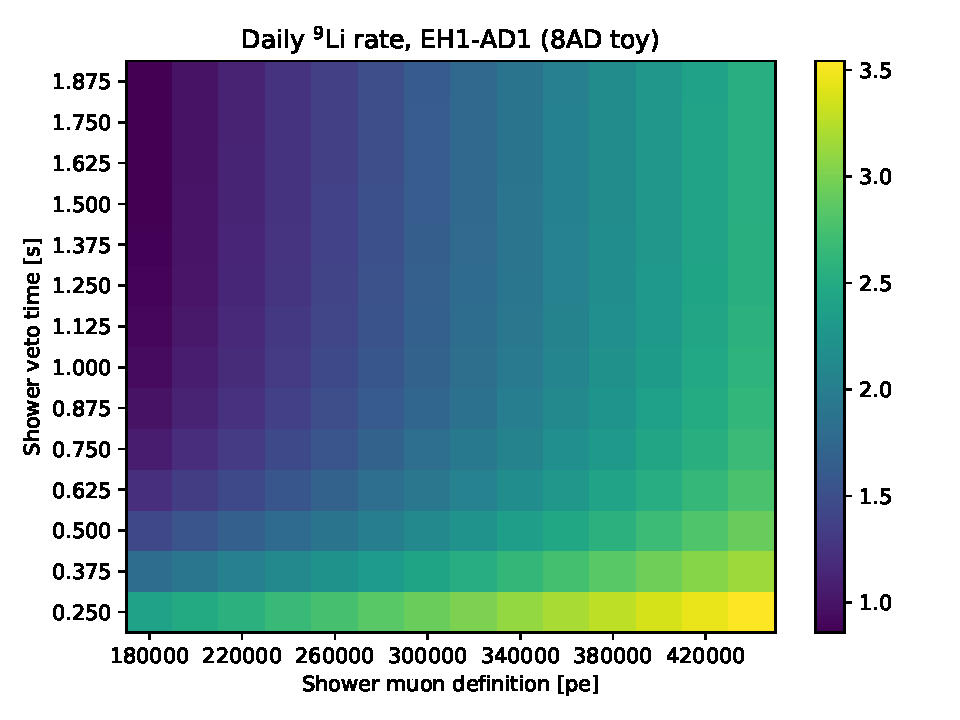
\includegraphics[scale=0.5]{CutVary/ShowerVeto/li9_bkg.eh1_ad1.8ad.pdf}%
  \end{minipage}%
  \begin{minipage}{0.5\linewidth}%
    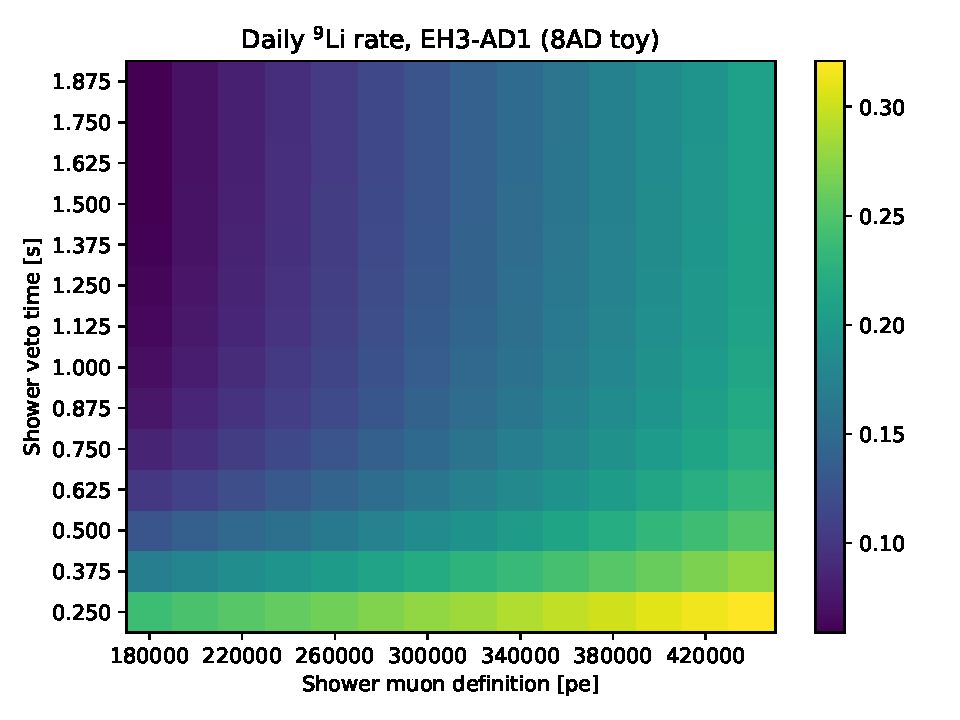
\includegraphics[scale=0.5]{CutVary/ShowerVeto/li9_bkg.eh3_ad1.8ad.pdf}%
  \end{minipage}%
  \caption{$^9$Li rate as a function of the shower veto parameters, for a near hall AD (left) and a far hall AD (right).}
  \label{fig:cutVaryVetoEffLi9Rates}
\end{figure}

The toy MC implementation of this study, then, requires taking the \texttt{Theta13} file produced by the nominal selection, and adjusting the veto efficiency, the $^9$Li rate, and its uncertainty. The veto efficiency correction is described in the following section. For the $^9$Li rate and uncertainty, we simply load the \texttt{Li9Calc} class from the IBD selector, as described in \autoref{sec:bkgCosmo} and feed it the modified veto parameters, producing the $^9$Li rates exemplified in \autoref{fig:cutVaryVetoEffLi9Rates}. Once the \texttt{Theta13} file has been thus modified, the toy MC will generate toy spectra that properly account for the expected effects on the veto efficiency and $^9$Li rate.

\subsection{Veto efficiency calculation}%
\label{sec:cutVaryMuVetoEff}

In order to use the toy MC for predicting and validating the data-driven optimization of the shower muon veto, we must provide the overall muon veto efficiency as an input to the toy MC (and subsequently to the fitter). During the analysis of real data, the veto efficiency is computed as one of the outputs of the IBD selection. In principle, then, for the toy MC study we could simply run the IBD selection, with the desired veto parameters, in order to obtain the time-averaged efficiency for a given definition of the veto. However, this is computationally expensive, and more importantly, it would be ideal for the toy MC cross check to be as decoupled as possible from the IBD selection and its associated data. Thus, we seek an independent method of determining the muon veto efficiency.

The veto efficiency is, naturally, a function of the muon rate. In particular, it depends on the rates of the three types of muons: water pool, AD, and shower. The first step, then, is to measure these rates, while taking care to avoid double counting due to retriggers and multi-detector muons. For this purpose, a ``muon selector'' was written to extract all of the muon events in our dataset. This is the one place where actual data enters this process, but the code is independent of the IBD selection's second stage, where IBD cuts (including the veto) are normally applied. Once the muon sample has been obtained, the rates of the three classes can be calculated. The final step is to calculate the efficiency, which requires a proper treatment of the possible overlap of veto windows between closely spaced muons. In what follows we describe these steps in detail and demonstrate that the results agree well with the veto efficiency obtained from the IBD selection.

\subsubsection{Muon rate measurement}%
\label{sec:cutVaryMuRate}

The objective of the muon rate measurement is to obtain, for each AD, two results: First, the rate of \emph{water pool-only} muons (i.e., those muons which produced a ``WP muon'' trigger without an associated ``AD muon'' trigger), and second, the spectrum (in terms of charge or energy) of those muons that triggered the AD\@. Given that the AD/shower veto windows are longer than the WP window, any AD+WP muon should be regarded as a single AD muon. The measurement of the AD muon \emph{spectrum}, rather than the total rate, is important because it enables a breakdown into ``shower'' and ``non-shower'' AD muons, which carry different veto windows, and it makes this breakdown possible while varying the shower muon definition, without requiring a re-run of the muon selection.

The muon selector runs on the output of the first stage of the IBD selection, i.e., the pre-selection, which does not depend on the IBD selection cuts. In particular, the muon selector reads the contents of the \texttt{muons} tree, which simply contains basic information (time, detector, and charge or energy) for each WP trigger with more than 12 above-threshold PMTs, and each AD trigger with more than 3000 p.e.\ of charge. We collectively refer to these events of muon-like triggers.

If we were to naively count the number of events of each type in the \texttt{muons} tree, we would overestimate the muon rates, for two reasons: Muons that trigger more than one detector must still be only counted once, and muon-induced retriggers must be discarded. The strategy for handling these subtleties is similar to the one described in \autoref{sec:bkgLi9MuonSel} for the muon selection used in the $^9$Li rate study:

\begin{itemize}
\item No distinction is made between the inner and outer water pools.
\item If a WP muon occurs less than 15~\us\ after an AD muon, it is discarded in favor of the AD muon.
\item If a WP muon occurs less than 5~\us\ after another WP muon (which, in practice, will always be in the other pool), and the number of hit PMTs is greater than the previous one, this muon replaces the previous one.\footnote{This reflects the fact that the IBD selection's muon veto simply requires one pool, and not necessarily both, to be above-threshold.}
\item If a WP muon occurs between 5 and 15~\us\ after another WP muon, it is discarded as a retrigger.
\item If an AD muon occurs less than 15~\us\ after another muon in the same AD, it is discarded as a retrigger.
\item If an AD muon occurs less than 5~\us\ after a WP muon, the WP muon is discarded in favor of the AD muon.
\end{itemize}

Each final ``merged'' muon produced by this procedure is stored in a histogram binned according to the number of hits (for WP muons) or the charge (for AD muons). It should be noted that there is a separate histogram of WP muons for each AD, even though all ADs in a hall share the same water pools. This is because an AD muon will override a WP muon, but a given muon will not necessarily pass through every AD, so the WP muon will still be counted for those ADs which do not see an associated AD muon.

\begin{comment}
  XXX local slides from mid-late Oct for retrigger plots. See misc_ana/MuonVetoEff/condenser4retrig.

Are our efficiencies biased because we don't count for the'' `muon multiplicity efficiency' coming from being falsely ignored as a retrigger?
\end{comment}

Using the histograms of WP and AD muons, the rates of the three muon classes can be calculated: First, the number of WP(-only) muons is determined by integrating the WP histogram for \texttt{nHit}$> 12$, while the number of (non-shower) AD muons is the integral of the AD histogram from 3000 PE to the shower threshold, and the number of shower muons is the above-threshold integral. These counts are then divided by the total livetime to obtain the three rates.

\subsubsection{Efficiency from the rates}
\label{sec:cutVaryMuVetoEffFromRates}

The final step is to calculate the veto efficiency from the three rates. Although the three muon classes are simple independent Poisson processes, it is difficult to calculate the veto efficiency analytically, given the possibility of overlapping veto windows between and within the three classes. On the other hand, it is trivial to simulate the processes, and the simulated veto windows can then simply be added (after removing overlaps) to determine the total vetoed time and hence the efficiency. For the sake of validation, three different approaches were tested, all with consistent results:

\begin{itemize}
\item A ``shotgun'' toy MC that generates $N$ (rate $\times$ time) random muons (of each type) distributed in time according to the uniform distribution, before sorting and merging them
\item A ``sequential'' toy MC that uses the relative rates to determine the type of the ``next'' muon, and the exponential distribution to determine the time to it
\item A ``parallel'' toy MC in which the three processes independently generate random samples of the time-to-next (i.e.\ exponential) distributions, with the events then sorted and merged. This version generated output files in the same format as the pre-selector, so the actual second-stage IBD selection could be run on them, to verify that our window-adding calculation agrees with that in the IBD selector.
\end{itemize}

\begin{figure}[ht]
  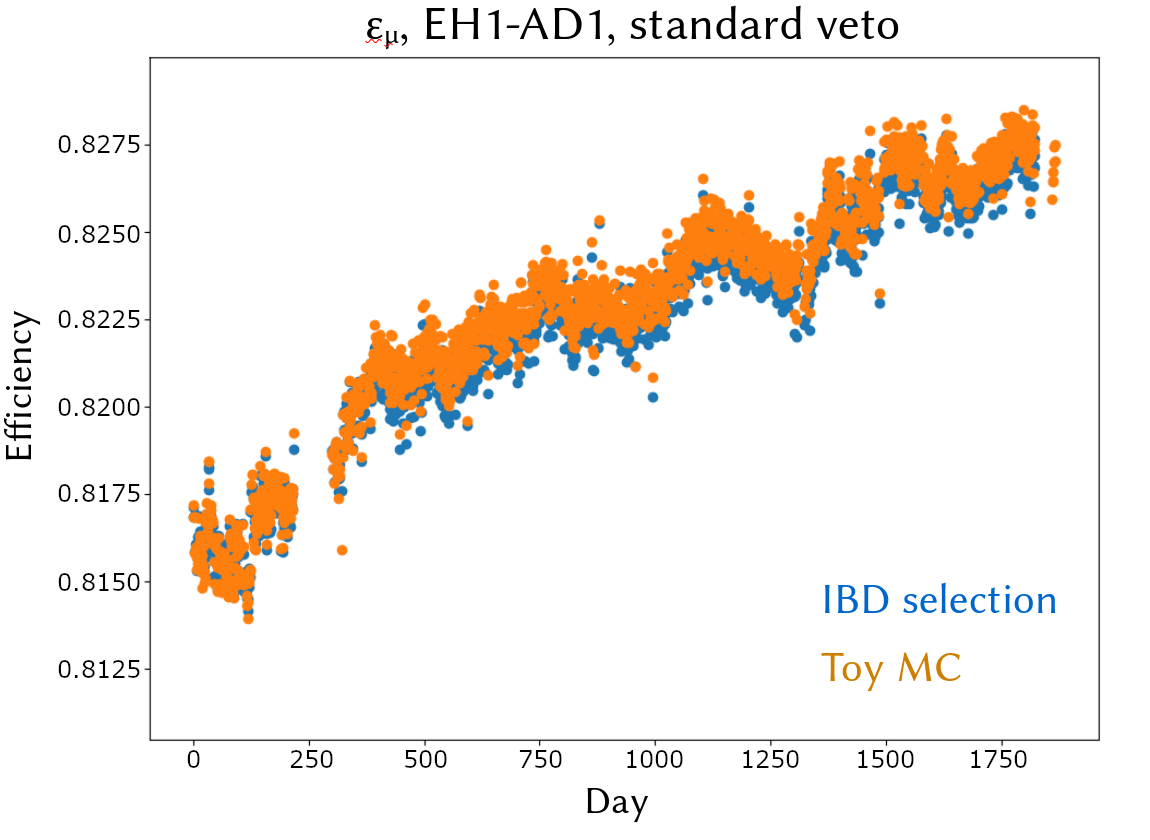
\includegraphics[scale=0.5]{CutVary/ShowerVeto/vetoEffCompare.png}
  \caption{Daily muon veto efficiency in EH1-AD1, both as reported by the IBD selection (by summing veto windows) and as calculated using the measured rates in the toy simulation.}
  \label{fig:cutVaryVetoEffCompare}
\end{figure}

\begin{figure}[ht]
  \begin{minipage}{0.5\linewidth}%
    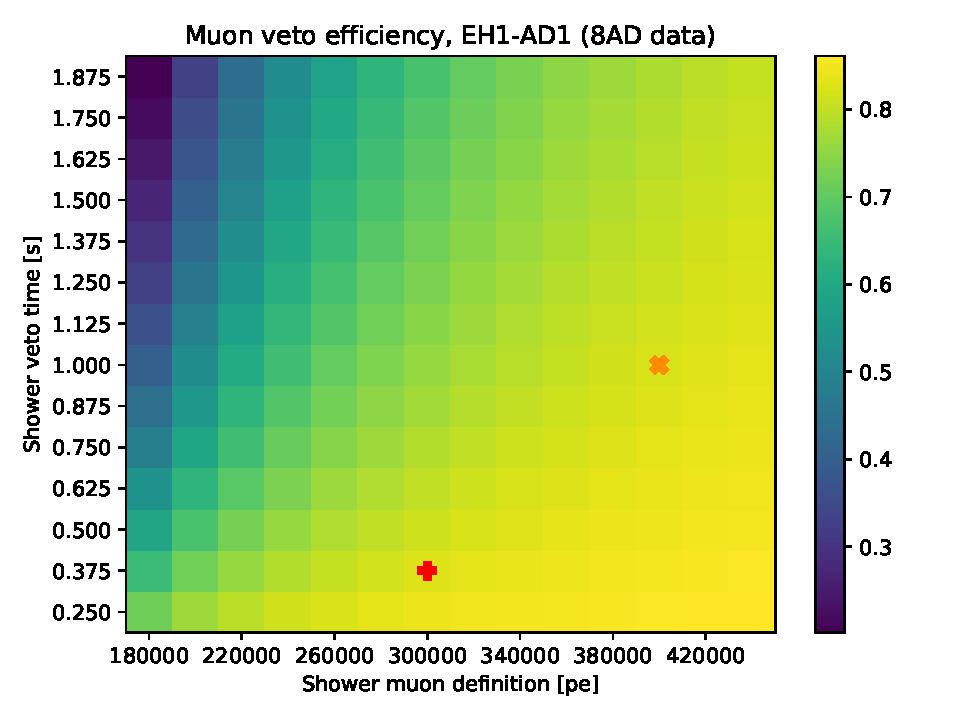
\includegraphics[scale=0.5]{CutVary/ShowerVeto/veto_eff.eh1_ad1.8ad.pdf}%
  \end{minipage}%
  \begin{minipage}{0.5\linewidth}%
  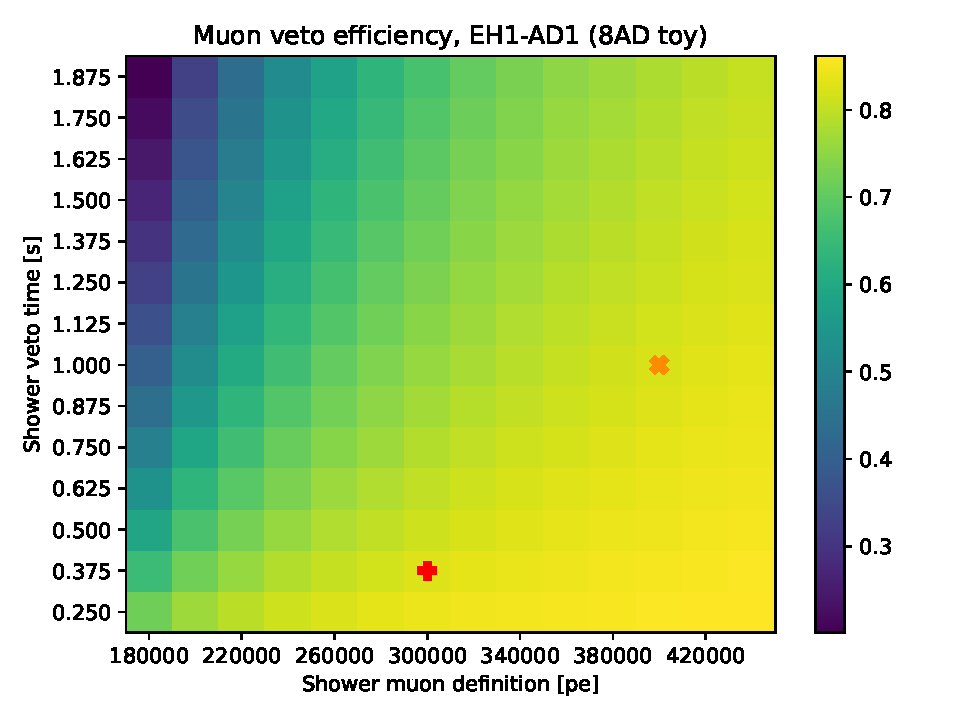
\includegraphics[scale=0.5]{CutVary/ShowerVeto/veto_eff.eh1_ad1.8ad_toymc.pdf}%
  \end{minipage}%
  \caption{Veto efficiency as a function of shower veto parameters in EH1-AD1 as determined by the IBD selection (left) and the rate measurement and simulation (right).}
  \label{fig:cutVaryVetoEff2dNear}
\end{figure}

\autoref{fig:cutVaryVetoEffCompare} shows the daily efficiency of the nominal muon veto, both as reported by the IBD selection, and by performing the calculation above using the rates measured from data. As can be seen, there is a very small bias (on the order of 0.02\%) inherent in this approach. This is unsurprising, given that the IBD selection does not discard muon retriggers, which can therefore extend the veto window by O(10~\us). In any case, this bias is not large enough to meaningfully impact the toy MC study of the shower veto\footnote{And the whole purpose of the toy MC study is merely to show that we don't expect any variation of the fit results as we vary the veto parameters.}. \autoref{fig:cutVaryVetoEff2dNear} compares the dependence of the efficiency upon the two shower veto parameters, as determined both by running the full IBD selection, and by using the above calculation on the muon rates measured by the nominal selection. Excellent agreement can be seen.

Having thus determined the expected veto efficiency for a modified shower veto, this value can be substituted into the \texttt{Theta13} file, along with the predicted $^9$Li rate. The toy MC can then be run as usual in order to generate the covariance and detector response matrices, etc., and then the Asimov toy spectra are fed to the fitter in order to extract the oscillation parameters. Meanwhile, for fits to data, the \texttt{Theta13} file is taken directly from the output of the IBD selection, and the fitter receives the prompt spectra from the data sample. In both cases, the toy samples (and hence the covariance matrices) are generated under the assumption of ``nominal'' oscillation parameters, namely $\SinSq = 0.084$ and $\Dmsqee = 0.00248$\footnote{As the covariance matrix has been shown to vary little under changes of the assumed oscillation parameters, we do not attempt to make the process more ``self-consistent'', such as by using an iterative procedure in which the covariance matrices are regenerated using the best-fit parameters, the fit is repeated, and so forth until convergence.}. In the following sections we discuss the fit results for both the toy and the real data samples.

\begin{comment}
Regarding results: Don't comment on ``structure'' until we've regenerated the 2D plots using the fix to SinglesCalc::calcSinglesHz. (Accidentals rate might have been biased, throwing off the fit.)
\end{comment}

\subsection{Fit results}%
\label{sec:cutVaryMuVetoDataResults}

\begin{figure}[ht]
  \begin{minipage}{0.5\linewidth}%
    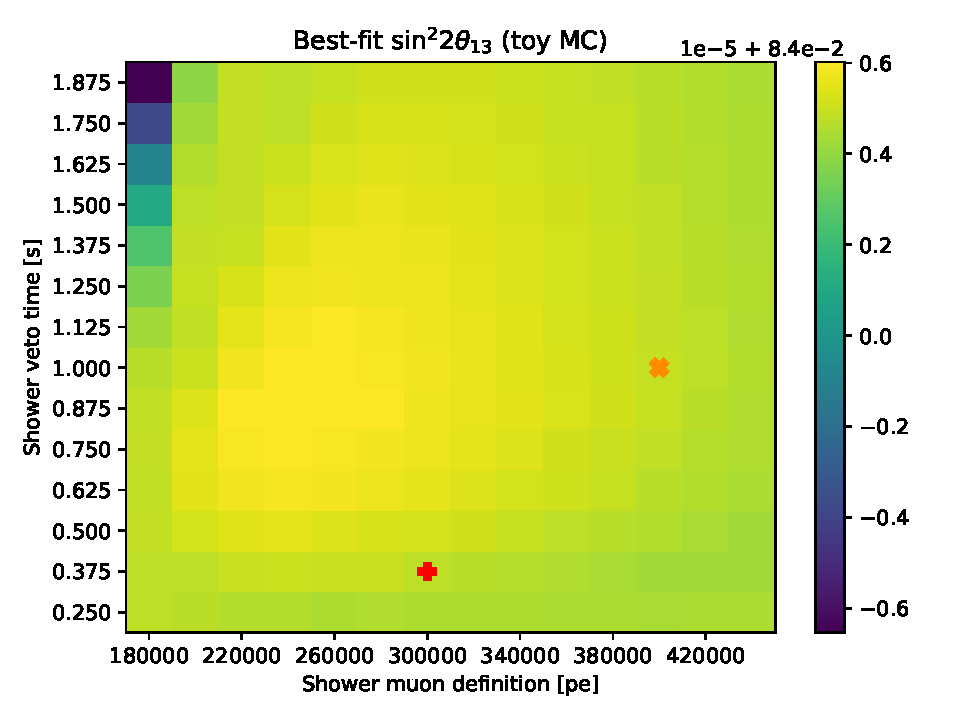
\includegraphics[scale=0.5]{CutVary/ShowerVeto/s2t_mid_toymc.pdf}%
  \end{minipage}%
  \begin{minipage}{0.5\linewidth}%
    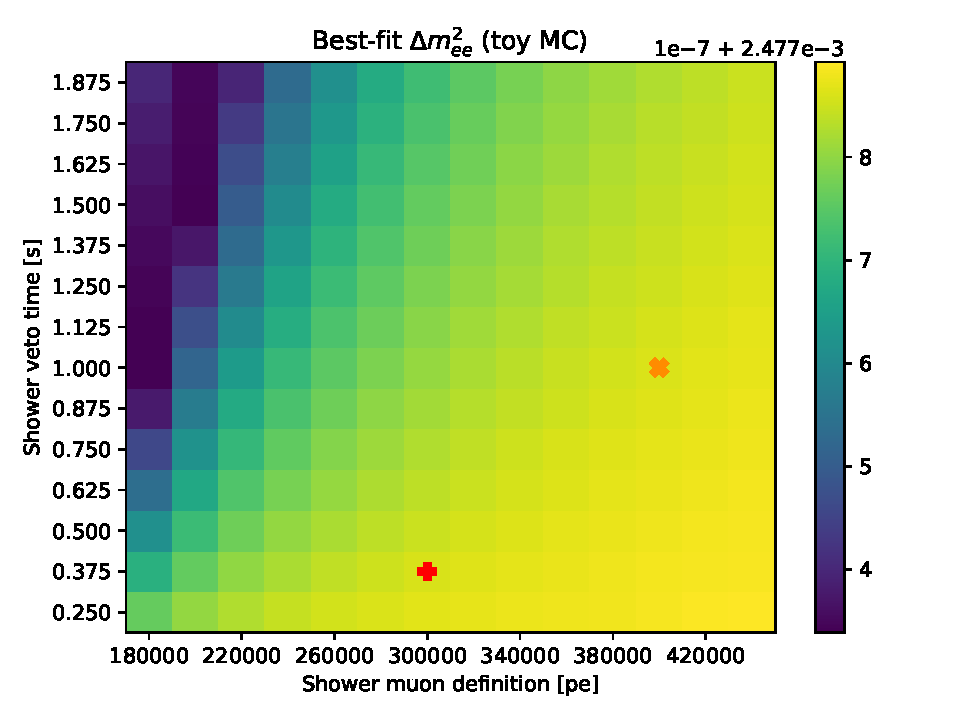
\includegraphics[scale=0.5]{CutVary/ShowerVeto/dm2_mid_toymc.pdf}%
  \end{minipage}%
  \caption{Results of oscillation fit to toy samples as a function of the shower veto parameters. On the left is $\SinSq$ and on the right is $\Dmsqee$.}
  \label{fig:cutVaryVetoEffToyResults}
\end{figure}

Toy samples were produced and fit in a uniform 14x14 grid of shower veto parameters, with the charge threshold ranging from 1.8e5 to 4.4e5 photoelectrons, and the veto time ranging from 0.25 to 1.875 seconds. \autoref{fig:cutVaryVetoEffToyResults} shows the results of the fits. The variation is on the order of 0.01\%, which is far below the scale of the analysis's uncertainty, and is likely attributable to rounding error of some kind. Thus, as expected, the toy MC predicts essentially no variation in the results of the oscillation analysis when the shower veto is varied.

\begin{figure}[ht]
  \begin{minipage}{0.5\linewidth}%
    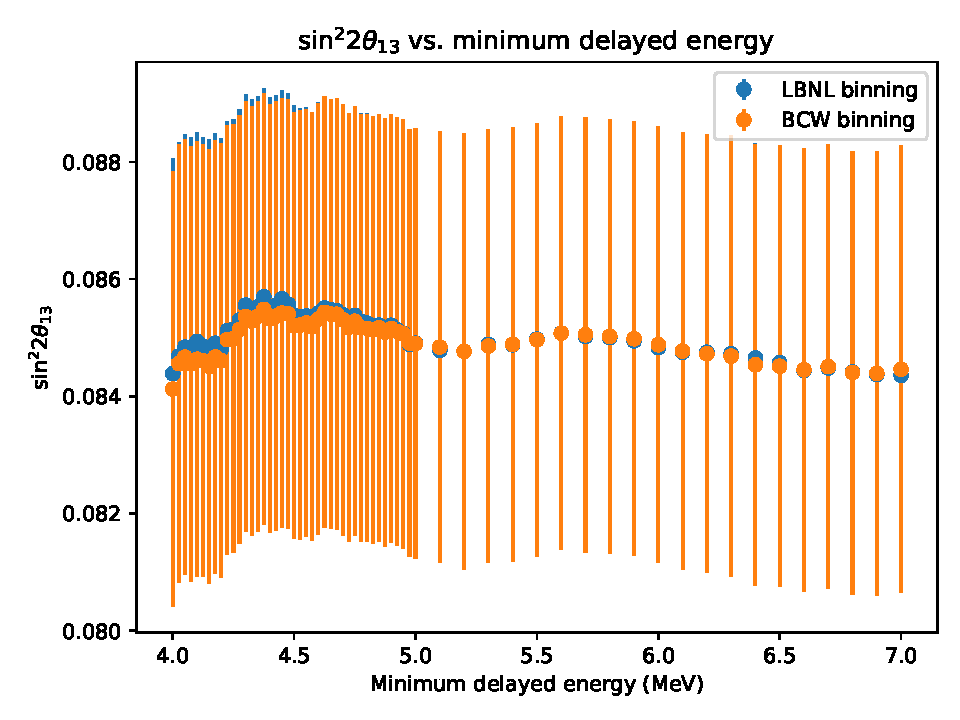
\includegraphics[scale=0.5]{CutVary/ShowerVeto/s2t_mid.pdf}%
  \end{minipage}%
  \begin{minipage}{0.5\linewidth}%
    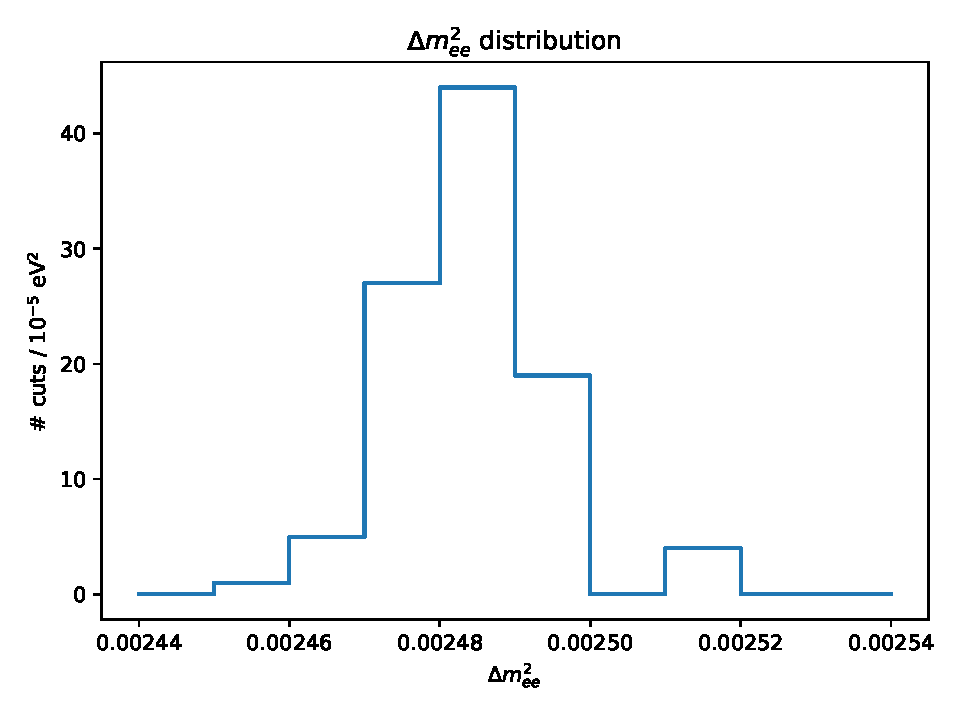
\includegraphics[scale=0.5]{CutVary/ShowerVeto/dm2_mid.pdf}%
  \end{minipage}%
  \caption{Results of oscillation fit to P17B data as a function of the shower veto parameters. Note different scale compared to \autoref{fig:cutVaryVetoEffToyResults}. On the left is $\SinSq$ and on the right is $\Dmsqee$.}
  \label{fig:cutVaryVetoEffDataResults}
\end{figure}

\autoref{fig:cutVaryVetoEffDataResults} shows the results of running the IBD selection and fitter on the P17B dataset, on the same grid of veto parameters as used in the toy MC study. In this case we see a greater degree of variation, which is unsurprising given that, in data, modifying the shower veto will produce statistical fluctuations, while this effect is abasent for the toy MC. Nonetheless, in a large region of parameter space, including both the LBNL and IHEP nominal vetoes, the fit is acceptably stable. Significant deviations are observed only on the left edge, where the loose definition of a shower muon results in an unreasonably low veto efficiency.

\begin{figure}[ht]
  \begin{minipage}{0.5\linewidth}%
    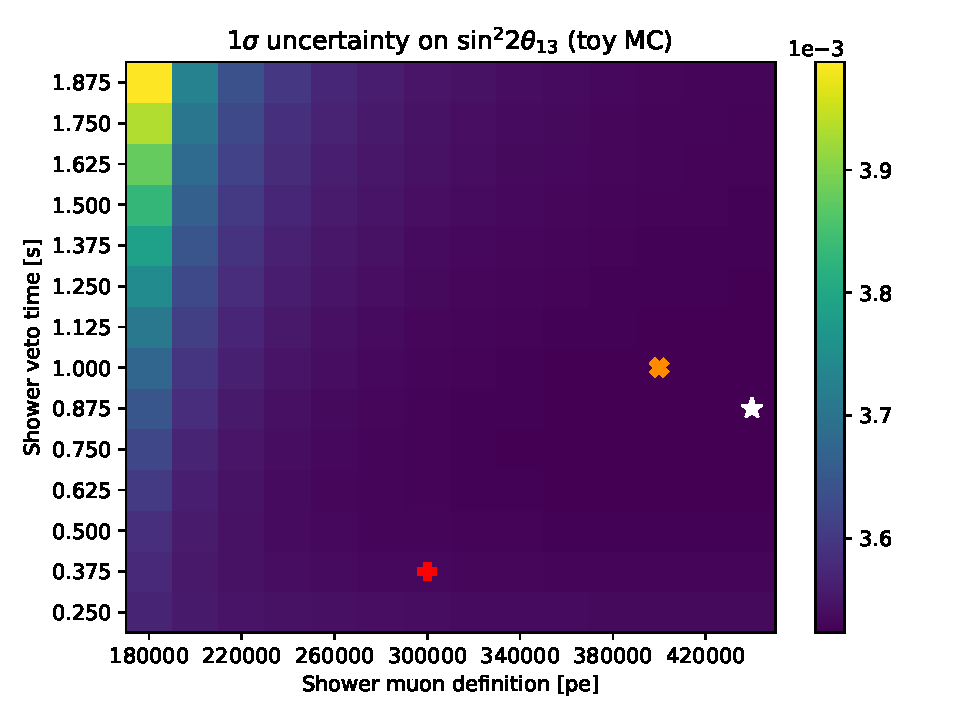
\includegraphics[scale=0.5]{CutVary/ShowerVeto/s2t_unc_toymc.pdf}%
  \end{minipage}%
  \begin{minipage}{0.5\linewidth}%
    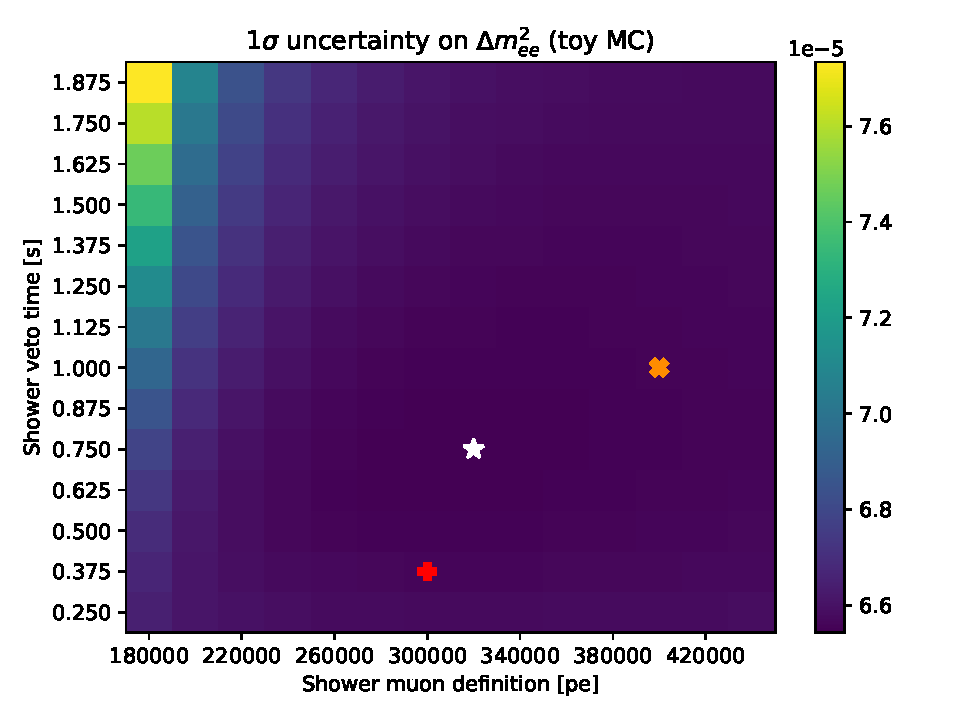
\includegraphics[scale=0.5]{CutVary/ShowerVeto/dm2_unc_toymc.pdf}%
  \end{minipage}%
  \caption{The fitter's reported uncertainty on $\SinSq$ (left) and $\Dmsqee$ (right) for fits to toy samples.}
  \label{fig:cutVaryVetoEffToyUnc}
\end{figure}

\begin{figure}[ht]
  \begin{minipage}{0.5\linewidth}%
    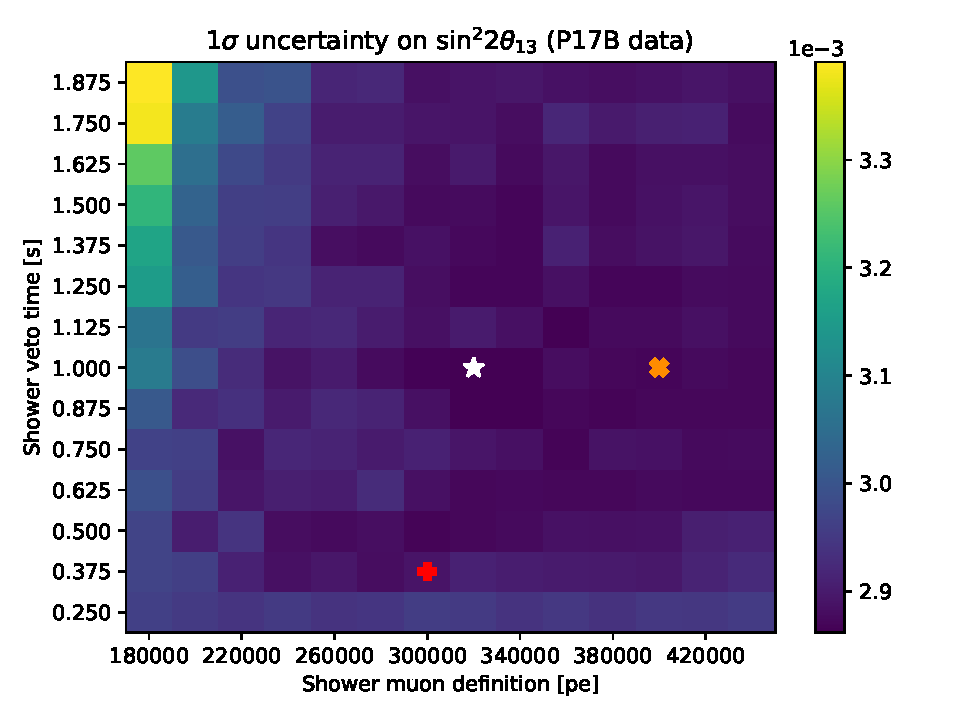
\includegraphics[scale=0.5]{CutVary/ShowerVeto/s2t_unc.pdf}%
  \end{minipage}%
  \begin{minipage}{0.5\linewidth}%
    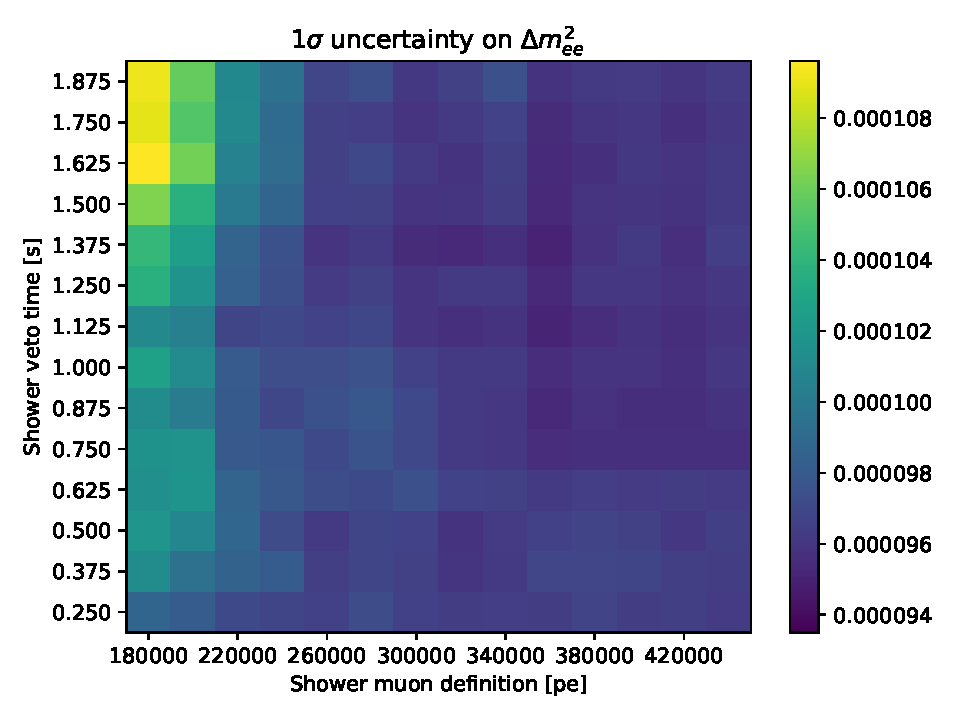
\includegraphics[scale=0.5]{CutVary/ShowerVeto/dm2_unc.pdf}%
  \end{minipage}%
  \caption{The fitter's reported uncertainty on $\SinSq$ (left) and $\Dmsqee$ (right) for fits to P17B data.}
  \label{fig:cutVaryVetoEffDataUnc}
\end{figure}

Although the toy and data fits showed very disparate scales of variation in the best-fit oscillation parameters, the variation in the reported fit uncertainty was more consistent between the two, as shown in \autoref{fig:cutVaryVetoEffToyUnc} and \autoref{fig:cutVaryVetoEffDataUnc}. As expected, the toy MC predicts a small but non-negligible amount of variation in the uncertainty, due to the aforementioned effect of the shower veto on both the veto efficiency (i.e. signal statistics) and the $^9$Li rate. The fits to data indicate a slightly higher uncertainty overall, possibly due to statistical fluctuations in the data sample, but the same general pattern of increasing uncertainty toward the upper left of the grid. In any case, the key conclusion from both the toys and the data is that the nominal shower veto (using a threshold of 3e5 photoelectrons and a veto time of 0.4004~s) lies within a large, flat valley in the parameter space. We are free to vary the parameters within this region without consequence, but there is also nothing to be gained from it. The nominal ``LBNL'' shower veto, as well as the veto used by the alternative ``IHEP'' analysis (Analysis A in \cite{An_2017}, vetoing for 1~s on muons of 2.5~GeV, or about 4e5 PE), can therefore both be considered ``optimal'' in the sense that they both achieve near-minimum uncertainty.

Meanwhile, the LBNL and IHEP vetos both lie in regions in which there is little variation in the best fit for small perturbations of the veto parameters. Curiously, however, there is a O(0.5\%) difference between the best fit values of $\SinSq$ for the LBNL and IHEP parameters (holding constant the remaining cuts). XXX We'd hope that both the LBNL and IHEP points give closer results. We'll see when we regenerate. Ideally, we see that the LBNL and IHEP points both lie within a large region of minimally varying best-fit $\SinSq$. Curious about the effects of using BCW binning. We should do both, so 14x14x2 = 392 sel/fits.

\section{Minimum delayed energy}
\label{sec:cutVaryMinDelayed}

\begin{figure}[ht]
  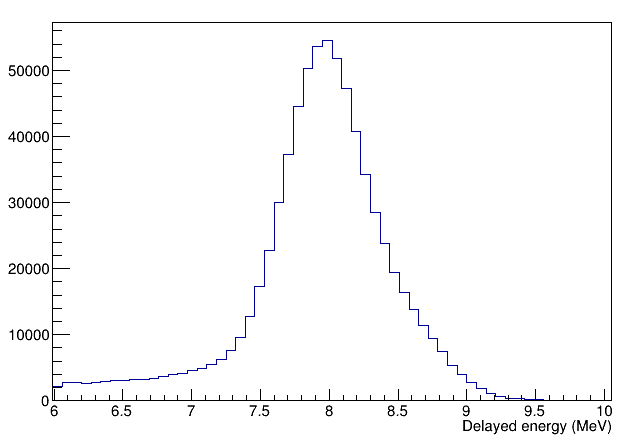
\includegraphics[scale=0.75]{CutVary/DelayedCut/eD_eh1ad1_8ad.png}
  \caption{The delayed energy spectrum of IBD candidates in EH1-AD1 during the 8AD period. Note the long tail to the left of the peak.}
  \label{fig:cutVaryDelCutDelSpec}
\end{figure}

In the reconstructed energy spectrum from nGd captures, there is a long and tall tail below the nominal cut of 6~MeV (\autoref{fig:cutVaryDelCutDelSpec}). This tail is populated by events in which one or more gammas ``leak'' beyond the active volume of the AD, leaving some of the initial energy unreconstructed. Estimates (XXX?) suggest that some 10\% of nGd captures fall below the 6~MeV cut. Due to this potential of gaining O(10\%) in signal statistics, it is worthwhile to explore the variation of the 6~MeV cut. Here we study modified delayed cuts ranging from 4 to 7~MeV.

Of course, there is a tradeoff: With an increase in signal comes an increase in backgrounds. For those correlated backgrounds that involve an actual delayed nGd capture ($^9$Li, fast neutrons, and $\alpha$-$n$), the rate will increase according to the same scaling factor as the signal rate. The AmC background possesses a different delayed energy spectrum (domninated by neutron captures in the AD's stainless steel vessel), and this spectrum is unknown (XXX); due to the small size of this background, we simply ignore it in the present discussion.

Although these correlated backgrounds do increase, the effect on the uncertainty is outweighed by the increase in signal statistics. Letting $k$ denote this scaling factor (i.e.\ the ratio of the new delayed efficiency to the old one):
\begin{align}
  \label{eq:cutVaryDelayedNcorrSigma}
  & N_{\mathrm{corr}} \equiv N_{\mathrm{obs}} - N_{\mathrm{bkg}} \\
  \implies & \sigma(N'_{\mathrm{corr}}) = \sqrt{k} \sigma(N_{\mathrm{corr}}) \\
  \implies & \frac{\sigma(N'_{\mathrm{corr}})}{N'_{\mathrm{corr}}} = \frac{\sqrt{k} \sigma(N_{\mathrm{corr}})}{k N_{\mathrm{corr}}} = \frac{1}{\sqrt{k}} \frac{\sigma(N_{\mathrm{corr}})}{N_{\mathrm{corr}}},
\end{align}
that is, even though there is an increase in the absolute uncertainty on the background-subtracted rate, the \emph{relative} uncertainty actually decreases. Therefore, if these were the only backgrounds at Daya Bay, it would be advantageous to use a delayed cut that is as low as possible.

Unfortunately, the accidental background is not as well-behaved. As shown in Fig.~XXX, the spectrum of delayed-like singles rises much more steeply below 5 (XXX?) MeV compared to the neutron capture spectrum, implying that the accidental background increases faster (percentage-wise) than the IBD rate. When this effect is large enough, the overall uncertainty on the background-subtracted IBD rate no longer decreases (as illustrated in \autoref{eq:cutVaryDelayedNcorrSigma}); instead, it \emph{increases}. In principle, then, it is the accidental background that serves to penalize overly loose definitions of the delayed energy cut.\footnote{In saying this, we are ignoring the possibility of new, unaccounted-for \emph{correlated} backgrounds appearing when we loosen the delayed cut. As we discuss later, this is in fact a likely issue.}

A further downside of loosening the delayed cut is that the multiplicity cut (DMC) efficiency is reduced, as we are now more likely to reject an IBD candidate on the basis of an ``extra'' delayed-like event in the 200~\us\ post-delayed window. However, this effect is outweighed by the increase in the efficiency of the delayed cut, as shown (XXX) by the following argument. (Use Eq 6 of the AccAndDMC chapter, etc.).

In theory, the toy MC should be able to capture and quantify the \emph{known} effects of varying the delayed cut, that is, the effects on the delayed cut efficiency (and by extension the signal statistics), on the accidentals, and on the nominal set of correlated backgrounds. We expect the toy MC to show no variation in the best fit (again, as a confirmation of the self-consistency of the toy MC / fitter system), but we do expect the uncertainty on the oscillation parameters to vary, based on the balance of the competing effects described above.

As with the shower muon veto, we carry out the toy MC study by taking the \texttt{Theta13} file from the nominal (i.e. 6~MeV) IBD selection, and altering those quantities that vary with the delayed cut. However, the toy MC does not have any built-in knowledge of how the signal efficiency and background rates vary with the delayed cut. As such, we must externally provide this knowledge, which we obtain from measurements down to 4~MeV of the neutron capture spectrum and the delayed-like singles spectrum. These measurements are described in Sec.~XXX.

When we perform fits to actual data using a modified delayed cut, the correct accidentals rate is automatically calculated by the IBD selector, and of course there is no need to apply (as in the toy MC case) a scaling factor to the raw signal rate. However, the correlated background rates must still be corrected using the same formalism as that applied for the toy MC. Furthermore, an additional complication arises from the fact that the ADs differ among themselves in the shape of their neutron capture spectra (Fig.~XXX). As a result, when we modify the delayed cut, the efficiency of this cut will not necessarily vary in unison among the ADs, possibly altering the measured near-far ratio. There are multiple ways to deal with this issue, and we discuss them further in Sec.~XXX. First, however, we discuss our treatment of the backgrounds.

\subsection{Treatment of backgrounds}
\label{sec:cutVaryDelayedCutBkgTreatment}

\subsubsection{Accidentals background}

For fits to actual data, the accidentals background is calculated by the IBD selector as described in XXX AccAndDMC. This calculation is valid for any delayed energy cut, so no further correction is necessary.

For fits to toy spectra, we use information from a special IBD selection run on the full P17B dataset. This special selection is simply the nominal selection with a loosened delayed cut of 4~MeV. From the spectrum of delayed-like singles measured by this selection, we can calculate the accidentals rate for any delayed cut of 4~MeV or greater. We do this by manually instantiating the relevant class from the IBD selector. The calculated rates are then substituted into the \texttt{Theta13} file.

\subsubsection{Correlated backgrounds}

For both toy and data fits, we use the same procedure. Since $^9$Li, fast neutron, and $\alpha$-$n$ events all include a delayed neutron capture, we can employ the neutron capture spectrum $S_n(E)$obtained from IBDs, whose extraction we describe in Sec.~XXX. For a delayed cut of $q$~MeV, the backgrounds are then simply scaled according to the ratio
\begin{equation}
  \label{eq:cutVaryDelCutCorrBkgScale}
  \frac{\int_q^{12} S_n(E)\,dE}{\int_6^12 S_n(E)\,dE}
\end{equation}

\subsection{Delayed cut efficiency}
\label{sec:cutVaryDelCutEff}

\begin{figure}[ht]
  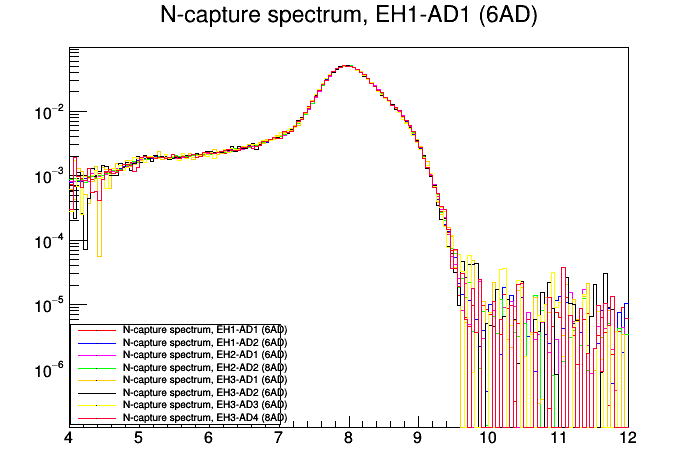
\includegraphics[scale=0.5]{CutVary/DelayedCut/overlay_h_ncap.png}
  \caption{Background-subtracted nGd capture spectra for the 8 ADs. Visually, the shape differences are practically undiscernable, but these small variations are nevertheless sufficient to produce an AD-dependent efficiency variation when the delayed cut is varied.}
  \label{fig:cutVaryDelCutSpecOverlay}
\end{figure}

As we show later (XXX), naively varying the delayed cut will cause a shift in the best-fit oscillation parameters (particularly $\SinSq$). This shift comes from slight AD-to-AD differences in the shape of the IBD delayed spectrum. In what follows, we will refer to this spectrum as the ``neutron capture'' or ``nGd'' spectrum.\footnote{Although the bulk of delayed triggers are indeed nGd captures, there is in fact a small peak around 5~MeV (Fig.~XXX) from neutron captures on carbon.} Due to these shape discrepancies, varying the delayed cut will cause its efficiency to vary by different amounts between the ADs.

In the published Daya Bay analyses, we have always assumed that all 8 ADs have the same delayed cut efficiency, to which we assign a nominal (and irrelevant) value of 0.88 in the \texttt{Theta13} file. However, from the observed differences in the nGd shape, it is clear that this assumption is inaccurate. Obviously, the efficiency of the 6~MeV cut cannot be measured by a direct comparison of the IBD rates between ADs, since this wouldn't account for all of the other effects (e.g., oscillation!) which affect the measured rate. However, the delayed cut efficiency\footnote{More accurately, the total detection efficiency, divided by those efficiencies (veto and DMC) that we treat individually.} \emph{could}, in principle, be measured by a fitter with 8 pull terms for the efficiencies and an additional pull term for the ``reactor antineutrino anomaly'' (the last of which already is included in the pull-based fitters used in the collaboration). Of course, including these 8 additional pulls could lead to a shift in the best-fit $\SinSq$, reflecting the fact that a particularly unfortunate combination of delayed cut efficiencies could be mistaken for an oscillation signal.

Our fitter, however, does not support pull terms. Instead, we could take the measured IBD rates, correct them for baseline and oscillation effects, and then take the ratios to, say, AD1, giving the 8 \emph{relative} efficiencies, normalized to AD1. Again, though, such an approach would suffer from the ambiguity between the effects of oscillation and unequal efficiencies. Thus, we make no attempt to perform a corrected rate-based measurement of the 6~MeV cut's efficiency. Instead, our approach is to measure the shape of the neutron capture spectrum as best as possible (as described in Sec.~XXX), and use that as our sole source of information on the efficiency of the delayed cut. Since our study extends down to delayed cuts of 4~MeV, so does our measurement of the neutron capture spectrum. The soft end of this spectrum includes both events from the nGd tail as well as nC captures.

Once the neutron capture spectrum has been measured, there are three ways it can be used (or not) to apply a correction factor to the IBD rate. We name and define these approaches as follows:

\begin{itemize}
\item \texttt{flat}: No correction. As in the official analysis, we simply assume that all ADs have the same delayed cut efficiency, for all values of the cut.
\item \texttt{relative}: We integrate the spectrum from $E_{\mathrm{cut}}$ to 12~MeV, and divide by the integral from 6 to 12~MeV. Thus, when $E_{\mathrm{cut}} = 12$~MeV, we reproduce the official analysis.
\item \texttt{absolute}: We again integrate from $E_{\mathrm{cut}}$ to 12~MeV, but this time we divide by the total integral of the measured spectrum (i.e., from 4 to 12~MeV).
\end{itemize}

The \texttt{flat} method is obviously the simplest, and as we shall show (XXX), it produces the aforementioned shifts in $\SinSq$, demonstrating that the delayed cut efficiency varies among ADs. Meanwhile, the advantage of the \texttt{relative} correction is that it allows us to show that we can obtain constant results as we move the delayed cut away from 6~MeV, provided that we correct for differences in the neutron capture shape. This proves that we understand and can account for the implications of varying the cut. However, the \texttt{relative} method says nothing about the size of the bias caused by the assumption of equal efficiencies at 6~MeV. This is where the \texttt{absolute} method provides insight. From the difference in the best-fit values of $\SinSq$ at 6~MeV between the \texttt{relative} and \texttt{absolute} methods, we can infer the scale of the aforementioned bias. This measurement is still uncertain, since there is a degree of arbitrariness from the choice of the lower cutoff (in our case, 4~MeV), but as we show, there are not many neutron captures with such low energy, so that variations around 4~MeV can be expected to have minimal effect.

We will show the results of applying all three methods, ultimately demonstrating excellent stability in $\SinSq$ when the relative method is applied between 5 and 7~MeV.

\subsubsection{Measurement of neutron capture spectra}
\label{sec:cutVaryDelCutSpecMeas}

Before we can integrate the neutron capture spectrum, we must, of course, measure it for each AD. It would be incorrect to use the raw delayed spectrum from the IBD candidates, since this includes contributions from backgrounds. Fortunately, all of the correlated backgrounds (except AmC, which we neglect due to its small rate) feature a neutron capture as the delayed event. On the other hand, accidental backgrounds will be drawn from the spectrum of delayed-like singles, which has a different shape from the neutron capture spectrum. Fortunately, both this spectrum and the accidentals rate can be measured quite accurately, so that we can obtain our final measurement simply by taking the delayed spectrum of IBD candidates, and subtracting the delayed-like singles spectrum scaled by the accidentals rate.

Although we did not diverge from this overall method, we implemented it in three different ways:

\begin{itemize}
\item \texttt{original}: We performed a ``reference'' IBD selection using a delayed cut of 4~MeV, extracting the neutron capture spectrum as described above. For any subsequent IBD selection with arbitrary cuts, this reference spectrum was used to obtain the (\texttt{relative} or \texttt{absolute}) efficiency.
\item \texttt{calc-then-add}: Within each IBD selection, we perform a ``parallel'' IBD selection using the same cuts, except with a 4~MeV delayed cut. The \emph{daily} spectrum, and then the efficiency (both \texttt{relative} and \texttt{absolute}) are obtained from the parallel selection. For the efficiency in the total sample, we use the weighted mean of the daily efficiencies.
\item \texttt{add-then-calc}: Again we use the ``parallel'' 4~MeV selection, but we do not calculate the efficiency on a daily basis. Rather, we add the daily neutron capture spectra in order to obtain the spectra for the full dataset, and then calculate the efficiency from these total spectra.
\end{itemize}

\begin{figure}[ht]
  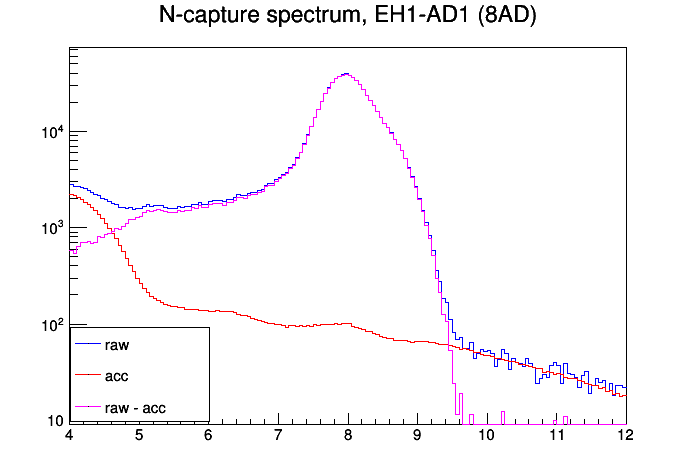
\includegraphics[scale=0.5]{CutVary/DelayedCut/ncap_log_8ad_eh1_ad1.png}
  \caption{Example of extracted neutron capture spectrum for EH1-AD1 in the 8AD period.}
  \label{fig:cutVaryDelCutNcapExample}
\end{figure}

For all cut variations we study \emph{except for the application of a vertex cut}, these three methods generally give equivalent results. However, when we apply a vertex cut (as discussed in \autoref{sec:cutVaryVertexCut}), there can be some variation in the shape of the neutron capture spectrum. The latter two methods were implemented so as to enable direct measurement of the efficiency for each cut, without recourse to a reference spectrum that may have the wrong shape. Although \texttt{calc-then-add} and \texttt{add-then-calc} are equivalent in principle, the former can suffer from division-by-zero in EH3 on days where there are no events in a given bin, so in practice we reject it in favor of \texttt{add-then-calc}.

\begin{comment}
In most of the results that follow, we show the outcome of using the \texttt{original} method, but the other methods give the same results. When we later discuss the application of vertex cuts, we will switch to the \texttt{add-then-calc} method (and will show the difficulties that result when attempting to use the \texttt{original} method).
\end{comment}

\subsection{Results}
\label{sec:cutVaryDelCutResults}

\begin{figure}[ht]
  \begin{minipage}{0.5\linewidth}%
    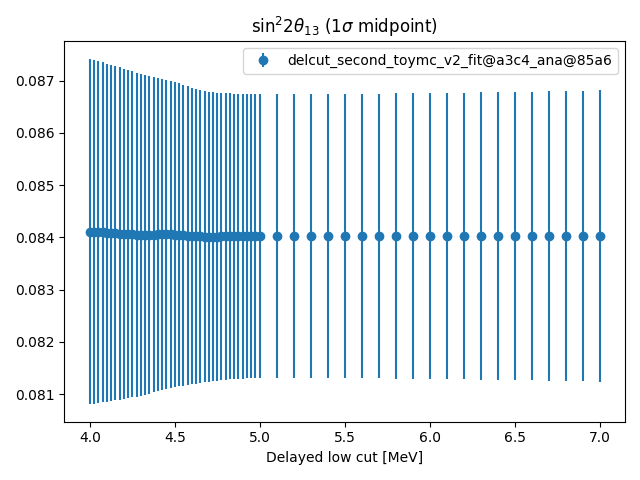
\includegraphics[scale=0.5]{CutVary/DelayedCut/s2t_mid_toymc.png}%
  \end{minipage}%
  \begin{minipage}{0.5\linewidth}%
    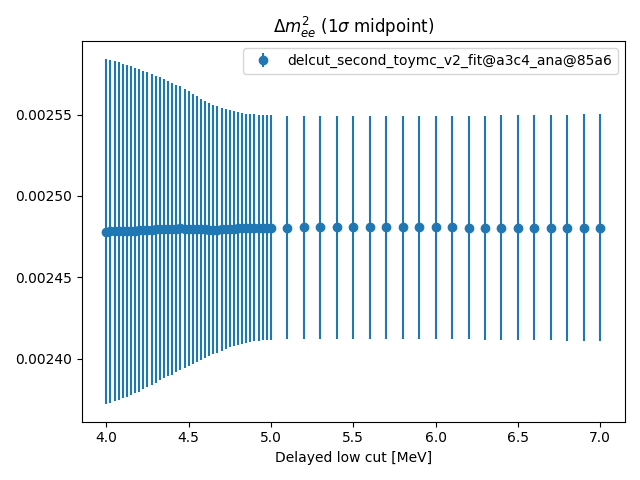
\includegraphics[scale=0.5]{CutVary/DelayedCut/dm2_mid_toymc.png}%
  \end{minipage}%
  \caption{Fit results from simulating the variation of the delayed cut in the toy MC.}
  \label{fig:cutVaryDelCutToyResults}
\end{figure}

As a sanity check, we begin by fitting toy samples. The toy MC does not simulate the delayed spectrum in any way whatsoever, but we can still adjust the efficiencies and background rates in the \texttt{Theta13} file to verify that the oscillation fit remains stable. In particular, for the results shown in \autoref{fig:cutVaryDelCutToyResults}, we inserted the delayed efficiencies calculated using the neutron capture spectra obtained from the nominal IBD selection (i.e., the \texttt{original} implementation), integrated according to the \texttt{relative} approach described previously. (TODO: Show results for flat/absolute. New impl???) The background rates were scaled as described in \autoref{eq:cutVaryDelCutCorrBkgScale}.

\begin{figure}[ht]
  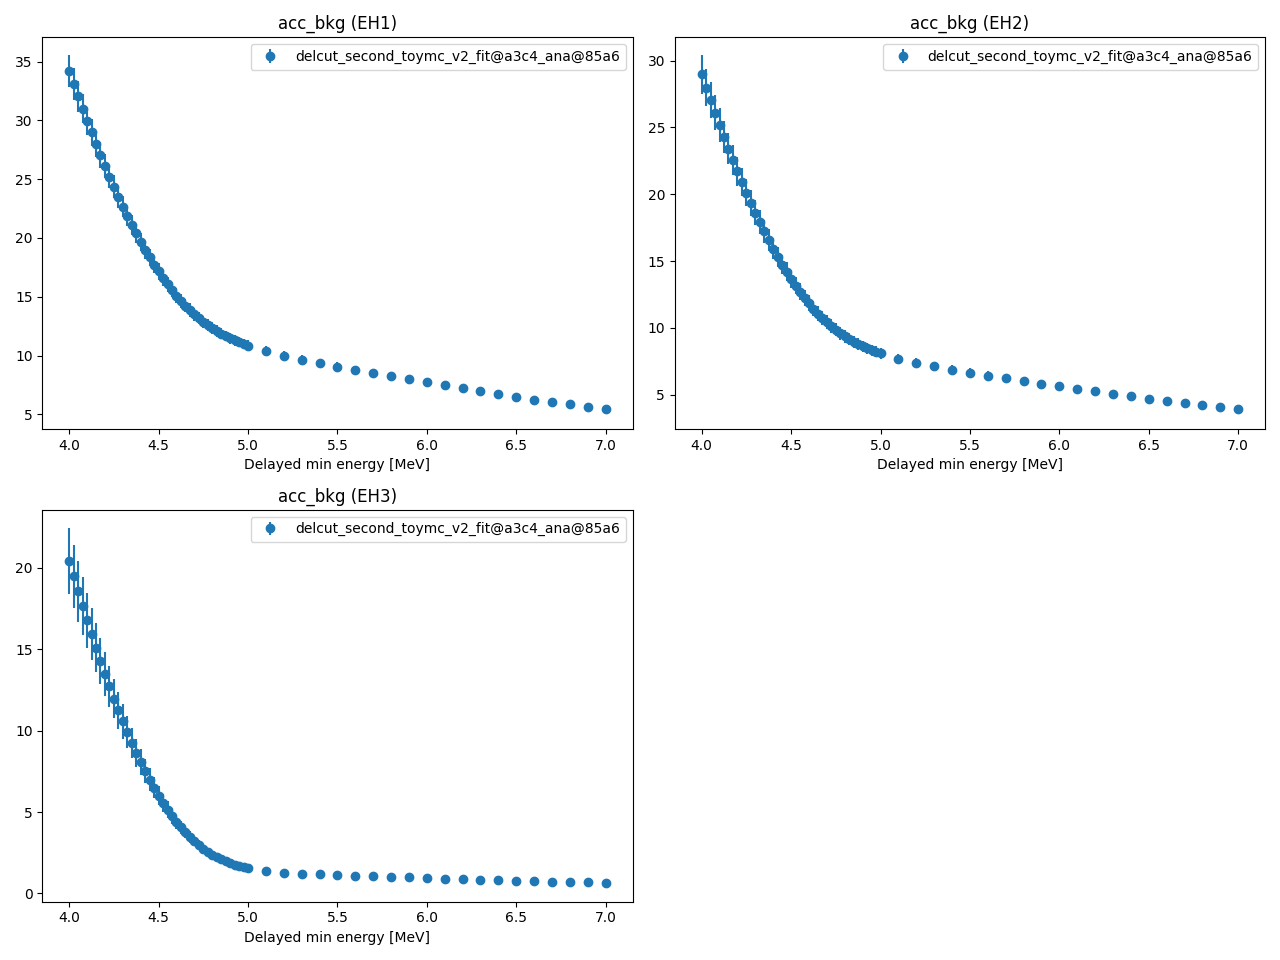
\includegraphics[scale=0.5]{CutVary/DelayedCut/acc_bkg.png}
  \caption{Accidental background rates as a function of the delayed cut. The full singles spectrum (from 0.7 to 12~MeV), taken from the nominal IBD selection, was used for the calculation.}
  \label{fig:cutVaryDelCutAccBkg}
\end{figure}

The toy MC results are shown in \autoref{fig:cutVaryDelCutToyResults}. They demonstrate the desired level of internal consistency, as both $\SinSq$ and $\Dmsqee$ are practically constant as the delayed cut is varied, with only a negligible increase in $\SinSq$ for the extreme case of a delayed cut near 4~MeV. We observe a $\sim$20\% increase in the uncertainty of both parameters near a delayed cut of 4~MeV, which can be attributed to the steep increase in accidental backgrounds, as shown in \autoref{fig:cutVaryDelCutAccBkg}.

\begin{figure}[ht]
  \begin{minipage}{0.5\linewidth}%
    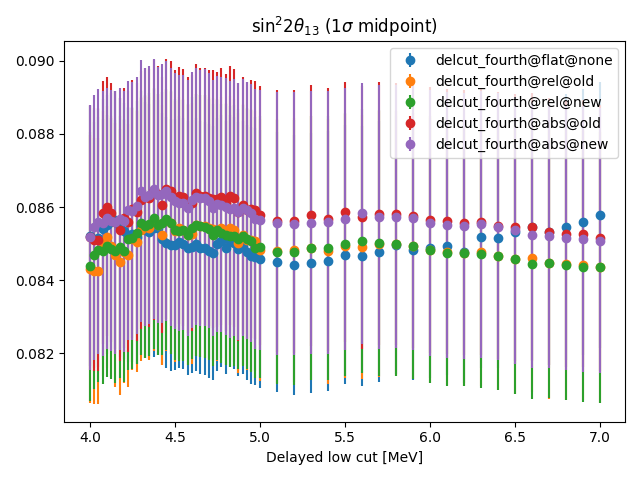
\includegraphics[scale=0.5]{CutVary/DelayedCut/s2t_mid_methcomp.png}%
  \end{minipage}%
  \begin{minipage}{0.5\linewidth}%
    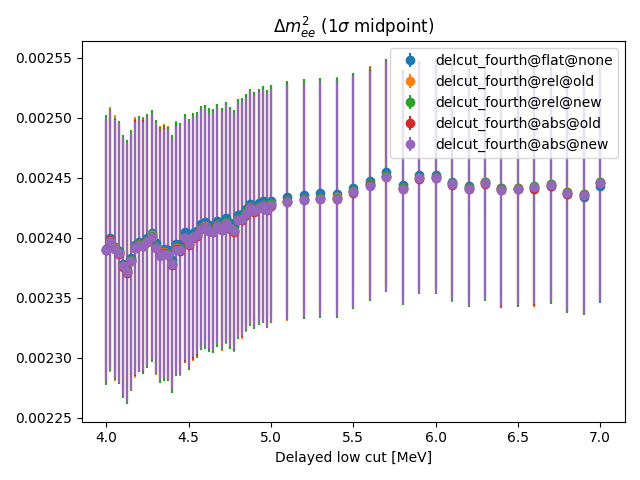
\includegraphics[scale=0.5]{CutVary/DelayedCut/dm2_mid_methcomp.png}%
  \end{minipage}%
  \caption{Fit results from actual data when varying the delayed cut. Shown are five different methods of measuring and correcting for the efficiency of the cut.}
  \label{fig:cutVaryDelCutDataResults}
\end{figure}

In \autoref{fig:cutVaryDelCutDataResults} we show the results of varying the delayed cut for the P17B data sample. In the legend, \texttt{old} refers to the \texttt{original} method of measuring the nGd spectrum, while \texttt{new} refers to the \texttt{add-then-calc} method, as described previously. Meanwhile, \texttt{flat}, \texttt{rel} and \texttt{abs} refer, unsurprisingly, to the \texttt{flat}, \texttt{relative} and \texttt{absolute} approaches for integrating the nGd spectrum.

The first thing to note is that there is almost no appreciable difference between \texttt{old} and \texttt{new}\footnote{This will not be the case when we apply a vertex cut, as shown later.}. Thus we focus on the differences between \texttt{flat}, \texttt{relative}, and \texttt{absolute}. In this discussion, we focus on $\SinSq$, since all five methods give essentially the same results for $\Dmsqee$. The \texttt{flat} approach shows by far the most variation in $\SinSq$, affirming the value of attempting to correct for AD-dependent variations in the delayed cut efficiency. Both the \texttt{relative} and \texttt{absolute} approaches are generally fairly stable; although some unexpected behavior is observed below 5~MeV, this amounts to only 10-20\% of the uncertainty. Unsurprisingly, an offset exists between the two approaches, as expected given that the \texttt{absolute} approach abandons the (arbitrary and unfounded) assumption that the ADs all have the same delayed efficiency at 6~MeV.

The behavior of $\Dmsqee$ below 5~MeV is surprising: There is a significant downtrend, culminating at approximately a third of the uncertainty. Moreover, two ``bumps'' are visible. These results suggest an unaccounted-for shape distortion for delayed cuts below 5~MeV. The most likely explanation is that this comes from backgrounds. Although the total background \emph{rate} calculation appears to remain generally correct, given the stability of $\SinSq$, the background shape is apparently being treated incorrectly. We further explore possible explanations of this effect in \autoref{sec:cutVaryVertexCut}. For the time being, we simply note that $\Dmsqee$ remains extremely stable between 5 and 7~MeV. Below 5~MeV, we are entering ``dangerous'' territory, where there was never any intention for the nGd analysis to tread, so anomalous behavior here is both unsurprising and unconcerning.

\begin{figure}[ht]
  \begin{minipage}{0.5\linewidth}%
    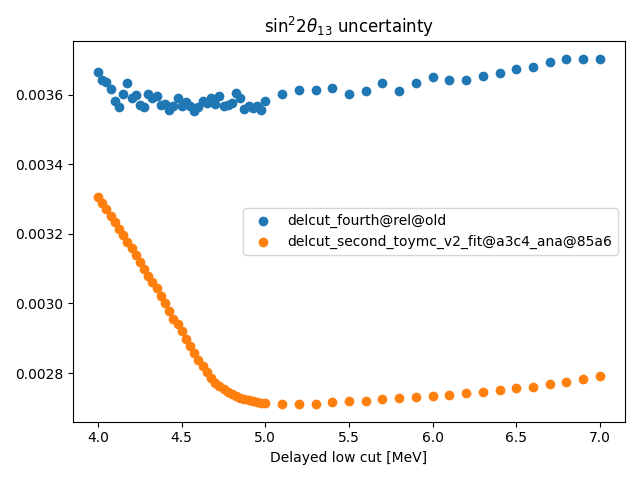
\includegraphics[scale=0.5]{CutVary/DelayedCut/unc_s2t_toyVsData.png}%
  \end{minipage}%
  \begin{minipage}{0.5\linewidth}%
    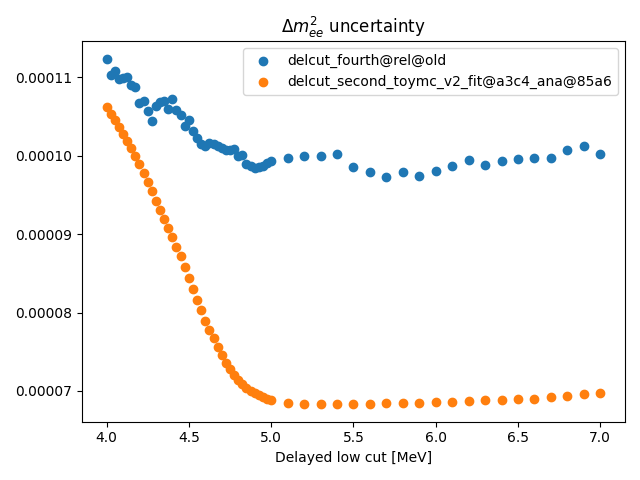
\includegraphics[scale=0.5]{CutVary/DelayedCut/unc_dm2_toyVsData.png}%
  \end{minipage}%
  \caption{Uncertainty as reported by the fitter under variations of the delayed cut for both the toy MC and P17B data.}
  \label{fig:cutVaryDelCutFitUnc}
\end{figure}

We end this section by showing the fitter's reported uncertainty under variations of the delayed cut (\autoref{fig:cutVaryDelCutFitUnc}). We do not expect perfect agreement here between the toy and the data, as the latter includes statistical fluctuations and systematic deviations, while the former uses the ``Asimov'' sample in which there are no statistical fluctuations and nominal assumptions are used for all systematics. Nevertheless, the overall scale of the uncertainty is in general agreement, as is the general form of a lopsided ``U'' shape. From these plots we can conclude that there is essentially no advantage, in terms of the fit uncertainty, to varying the standard 6~MeV cut.

\section{Minimum prompt energy}
\label{sec:cutVaryMinPrompt}

Unlike the delayed spectrum, the prompt spectrum of IBDs does not contain a long tail, so that varying the prompt cut is likely to have a smaller effect on the analysis, with minimal potential statistical gain. Although the minimum IBD energy deposition is 1.02~MeV (from positron annihilation), the finite detector resolution leads to the reconstruction of some events below this minimum energy. Since we can see that the prompt spectrum doesn't fall to zero at 0.7~MeV (Fig.~XXX), it is clear that events will be lost or gained upon variation of the cut. It is therefore worth verifying that the analysis is stable under such circumstances.

\emph{A priori,} there is no reason to assume that the prompt cut has the same efficiency (and $d\epsilon/dE_{\mathrm{cut}}$) across all ADs. Just as with the delayed cut, it is possible that we may need to apply corrections for the AD-dependent prompt efficiency. In that case, we could extract the prompt spectrum analogously to the case of the delayed spectrum, and then integrate it using either the \texttt{absolute} or \texttt{relative} methods.

Compared to the delayed spectrum, it may be possible to more accurately measure the absolute efficiency, given the lack of a long tail. Even though the rate of prompt-like singles rises very steeply around 0.7~MeV, the accidentals rate is bottlenecked by the rate of delayed-like singles, so the accidentals subtraction can still be performed accurately. However, the \emph{correlated} backgrounds each have their own externally supplied prompt spectra, which (as we describe XXX below) must be individually integrated (to scale the rate) and subtracted. Hence, the measured prompt spectrum could be skewed by any errors in the rates and spectra of the correlated backgrounds. Fortunately, the total rate of the correlated backgrounds is quite low, and in the case of the dominant one ($^9Li$), 0.7~MeV lies below its lower endpoint (XXX check and revise). We therefore don't expect the correlated backgrounds to pose a major difficulty in the prompt spectrum extraction.

The above discussion is irrelevant, however, because as we shall see, the \texttt{flat} method (in which we make no attempt to correct for the prompt efficiency) produces remarkably stable results. There is therefore no need to extract the prompt spectrum, so we will leave it at that.

When varying the prompt cut, then, the only adjustment we must make to the \texttt{Theta13} file is to correct the rates of the correlated backgrounds. Since we are in the possession of predicted prompt spectra $S_b(E)$ that extend down to 0~MeV for each correlated background $b$, we have all of the information needed. We simply take the nominal background rate (and uncertainty) and scale it according to the factor
\[
  \frac{\int_{E_{\mathrm{cut}}}^{12} S_b(E)}{\int_{0.7}^{12} S_b(E)}.
\]
The fitter, when subtracting the background, then takes $S_b(E)$, cuts it off at $E_{cut}$, normalizes it to the specified rate, and subtracts it from the raw prompt spectrum. This adjustment of the correlated backgrounds is applied for both the cases of fitting data and toy samples. There are no further subtleties related to the variation of the prompt cut.

As shown in Fig.~XXX, the toy MC predicts no shift in the best-fit oscillation parameters, as expected. Furthermore, there is no significant change in the total uncertainty, indicating that there is no obvious ``optimum'' prompt cut to use.

Meanwhile, Fig.~XXX shows the results of fitting actual data. Happily, there is no significant change in the best-fit values of $\SinSq$ and $\Dmsqee$ when we vary the prompt cut. Likewise, the uncertainty remains stable. Thus, with minimal effort, we have demonstrated that our analysis is stable against changes in the prompt cut, and that there is nothing suboptimal about the nominal cut of 0.7~MeV.

\section{Vertex cut}
\label{sec:cutVaryVertexCut}

\begin{comment}
  XXX Do our adjustments of background rates account for the fact that some backgrounds can occur in the GdLS+LS whereas others occur only in GdLS?

Accidentals -- Handled automatically, no adjustment, we're good
Li9, fast-n, alpha-n: Only in GdLS, ???
AmC: Both. R distribution unknown but probably ``lumpy''. Z probably like what we did.
\end{comment}

Since our analysis is based on nGd IBDs, the delayed events of the IBDs will all take place within the GdLS volume. Given the small (cm-scale) neutron diffusion distance, most of the prompt events will likewise occur in the GdLS\footnote{Those that don't are accounted for in the spill-in efficiency.}. The situation is the same for the three correlated backgrounds ($^9$Li, fast neutrons, and $\alpha$-n) that involve nGd captures.

Meanwhile, for accidental backgrounds, there is no correlation between the prompt and delayed vertices; most (but not all) of the delayed triggers will come from nGd captures (and thus lie within the GdLS), while there will be many prompt-like triggers in the LS as well as the GdLS. And finally, the AmC backgrounds will show a tight prompt-delayed correlation, but with a unique vertex distribution localized toward the top of the AD near the three ACUs.

Based on these facts, it is obvious why the official nGd analysis does not employ any cuts on the event vertices. Although there is nothing preventing us from requiring reconstructed vertices to lie within the GdLS volume (or any other fiducial volume), such a cut will gain only a small reduction of the accidental and AmC backgrounds. This small gain is outweighed by the risk of introducing an AD-dependent efficiency of the vertex cut, which can bias $\SinSq$ if it is not carefully measured and corrected for.

Nevertheless, it is worthwhile to explore the results of applying an arbitrary vertex cut \emph{(with an efficiency correction)}, if only as a demonstration of the robustness of our analysis and the reliability of the vertex reconstruction. Going beyond this motivation, a vertex cut can be useful in exploring the behavior of \emph{other} cuts. In particular, we recall that, as shown in Fig.~XXX, the best-fit value of $\Dmsqee$ trends downward as we reduce the delayed cut below 5~MeV. In Sec.~XXX, we hypothesized that an unaccounted-for correlated background, potentially originating from the AmC sources, may be responsible for this behavior. Given that AmC-associated events occur closer to the top of the AD, the application of (vertical) vertex cuts can provide a means of testing this hypothesis: If the AmC sources are indeed responsible, then the downard trend in $\Dmsqee$ should be lessened when we select events closer to the bottom of the AD\@.

For these reasons, we choose to go beyond the official analysis and explore the use of vertex cuts. When applying a vertex cut, care must be taken in two areas: the detection efficiencies and the background rates. As was mentioned, a vertex cut may not have the same efficiency among all ADs, so this efficiency must be measured and corrected for. The accidental background rate calculation, being based on the singles selection (to which we apply the same vertex cut), accounts for the vertex cut automatically. As for the correlated backgrounds, we must assume a particular vertex distribution for each background, and then calculate the percentage of the distribution that lies within our fiducial volume.

Throughout this study, we apply a given vertex cut to both the prompt and delayed vertex. This is to be distinguished from, say, the muon veto, which considers only the delayed trigger. We choose to cut on both triggers because it avoids the need to make an arbitrary choice between prompt and delayed, and it avoids the need to perform two separate singles selections with two different vertex cuts.

In the sections that follow, we first describe the measurement of the vertex cut efficiency and how we correct for it, followed by our adjustments of the correlated background rates. We then proceed to explore the effects of applying five different vertex cuts (three vertical and two cylindrical; see \autoref{tab:cutVaryVtxCutCutsTbl}) to the nominal selection, before extending to the case of modified delayed cuts, with the goal of gaining insight into the trends observed in $\Dmsqee$. We end by drawing what conclusions we can regarding those trends as well as the overall robustness of our analysis to vertex cuts, and whether the observed variations are consistent with our statistical uncertainty.

\subsection{Implementation details}
\label{sec:cutVaryVtxCutImplDet}

Within the IBD selection, the vertex cut is implemented using the vertex provided by the \texttt{AdSimple} reconstruction, after conversion from Cartesian coordinates to the natural cylindrical coordinate system of the AD. The cut involves four parameters, corresponding to the minimum and maximum acceptable radial and vertical coordinates. Both the singles selection and the IBD selection apply the cut, in the latter case to both the prompt and delayed triggers. Furthermore, when applying the multplicity cut, any ``extra'' triggers are ignored if they do not pass the vertex cut (i.e., such triggers will not cause the single/IBD candidate to fail the multipliticy cut). In effect, any (non-muon) trigger that fails to pass the vertex cut is completely excluded from the analysis.

\subsection{Efficiency calculation}
\label{sec:cutVaryVtxCutEffCalc}

Before going into the details of the efficiency calculation, it is worthwhile to demonstrate \emph{why} it is worthwhile to carry it out in the first place. First, we must define some vertex cuts to investigate. \autoref{tab:cutVaryVtxCutCutsTbl} lists five cuts along with the names we will use when referring to them in the remainder of this chapter. Using those definitions, Fig.~XXX shows the best-fit oscillation parameters obtained when applying these cuts without any efficiency correction. We expect some scatter, given that we are analyzing statistically independent subsamples.\footnote{More precisely, the three vertical cuts are statistically independent from each other, and likewise for the two radial cuts, but there \emph{is} a degree of overlap between each vertical and each radial cut. The overall point remains, however.}. Since we know that roughly half of the fit's uncertainty comes from statistics (as discussed in XXX fitting chapter), and since the vertical (radial) cuts approximately divide the sample into thirds (halves), we can estimate the statistical uncertainty on each subsample to be between $0.5\sqrt{2}$ and $0.5\sqrt{3}$ of the total (full sample statistical + systematic) uncertainty, i.e. 70--85\% of the total error bar. From Fig~XXX, it is apparent that the scale of the scatter is slightly larger than 1$\sigma$. While a mere statistical fluctuation cannot be ruled out, this result suggests that we should attempt to determine whether an AD-dependent efficiency variation may be playing a role (in which case a correction should be applied). As we will shortly show, when we measure the vertex efficiency, we do in fact find different values among the ADs, and applying a correction indeed reduces the scatter between the fit results.

\begin{comment}
(XXX note we haven't actually plotted the results of applying no efficiency correction. The scatter might be well above 1sigma in which case we need to reword the above.)
\end{comment}


\begin{table}[h]
  \begin{tabular}{lc}
    \toprule
    Name & Definition \\
    \midrule
    \texttt{zTopThird} & $z \in [0.5,\, 1.5]\,\mathrm{m}$ \\
    \texttt{zMidThird} & $z \in [-0.5,\, 0.5]\,\mathrm{m}$ \\
    \texttt{zBotThird} & $z \in [-1.5,\, -0.5]\,\mathrm{m}$ \\
    \texttt{rInside1000} & $r < 1\,\mathrm{m}$ \\
    \texttt{rOutside1000} & $r > 1\,\mathrm{m}$ \\
    \bottomrule
  \end{tabular}
  \caption{The five vertex cuts under investigation.}
  \label{tab:cutVaryVtxCutCutsTbl}
\end{table}

\begin{comment}
  TODO Try doing vertex efficiency with background subtraction. Oh wait we already do.
\end{comment}

\subsubsection{Procedure}
\label{sec:cutVaryVtxCutProc}

The vertex cut efficiency is determined by taking the ``corrected'' IBD rate obtained with the vertex cut, and comparing it to the corrected rate obtained from an IBD selection (the ``reference'' cut) which has no vertex cut but otherwise identical cuts. The meaning of ``corrected'' will be explained shortly. If the vertex cut is the only modification made to the nominal IBD selection, then we simply use the nominal selection as a reference; however, if we modify any other cuts (such as the delayed cut) while applying the vertex cut, we must perform a reference IBD selection with those same modifications (minus the vertex cut). This ensures that the measurement is not biased by any efficiency variation caused by the other modified cuts, which could occur if we simply used the nominal selection as the reference in all cases.

The corrected IBD rate $R_{\mathrm{corr}}$ is calculated straightforwardly: We simply take the total number of IBD candidates $N_{\mathrm{raw}}$, subtract the total predicted number of backgrounds, and divide by the livetime, the veto efficiency, and the multiplicity efficiency. Since the IBD selection's convention is to output the background prediction $R_{\mathrm{bkg}}$ as an efficiency- and livetime-corrected daily rate, we must undo these corrections before performing the subtraction. In summary:
\begin{align*}
  N_{\mathrm{bkg}} &= R_{\mathrm{bkg}} \cdot T \cdot \epsilon_\mu \cdot \epsilon_m\\
  R_{\mathrm{corr}} &= (N_{\mathrm{raw}} - N_{\mathrm{bkg}}) \;/\; (T \cdot \epsilon_\mu \cdot \epsilon_m)
\end{align*}

The efficiency of the vertex cut is then obtained by simply taking the ratio with respect to the reference selection:
$$ \epsilon_v = R_{\mathrm{corr}}^{\mathrm{cut}} \;/\; R_{\mathrm{corr}}^{\mathrm{ref}}. $$

\subsection{Background rate adjustment}
\label{sec:cutVaryVtxCutBkgRate}

In the preceding discussion of the efficiency calculation, the background rate $R_{\mathrm{bkg}}$ is itself implicitly a function of the vertex cut, and is thus different between the selection in question and the reference selection. This modified value of $R_{\mathrm{bkg}}$ must also, of course, be the one we use when subtracting the backgrounds during the oscillation fit. Here we discuss how the five background rates are affected by the use of a vertex cut.

\subsubsection{Accidentals}

The accidental background is calculated, as usual, directly from the prompt- and delayed-like singles rates obtained from the singles selection. Since we apply the same vertex cut in the IBD and the singles selection, the calculated accidentals rate automatically takes the vertex cut into account. No adjustment is therefore necessary.

\subsubsection{$^9$Li, fast neutrons, and $\alpha$-$n$}

These ``neutronic'' backgrounds are assumed to be uniformly distributed throughout the GdLS. Since fast neutrons arrive from above and stop inside the AD, some bias toward the top is expected, but this effect has been shown to be small (XXX cite; see Beda's email). Meanwhile, since $^9$Li-producing shower muons pass through the AD, no such bias is expected. Likewise, $\alpha$ activity is uniformly distributed throughout the AD.

Based on this uniformity assumption, we define a ``radial'' factor $f_r$ to account for the minimum and maximum radii accepted in the cut, and likewise a ``vertical'' factor $f_z$ corresponding to the minimum and maximum acceptable vertical coordinates. In order to account for the finite resolution of the vertex reconstruction, we ``extend'' the dimensions of the IAV by 200~mm in every direction, leading to the following definitions of the nominal minimum and maximum coordinates:
\begin{align*}
  r_{\mathrm{min}}^{\mathrm{nom}} &= \SI{0}{mm}\\
  r_{\mathrm{max}}^{\mathrm{nom}} &= \SI{1700}{mm}\\
  z_{\mathrm{min}}^{\mathrm{nom}} &= \SI{-1700}{mm}\\
  z_{\mathrm{max}}^{\mathrm{nom}} &= \SI{1700}{mm}.
\end{align*}

Since these backgrounds are not expected to occur outside the GdLS, we clamp the vertex cut parameters at the limits defined above:
\begin{align*}
  r'_{\mathrm{max}} &= \min(r_{\mathrm{max}}, r_{\mathrm{max}}^{\mathrm{nom}})\\
  z'_{\mathrm{min}} &= \max(z_{\mathrm{min}}, z_{\mathrm{min}}^{\mathrm{nom}})\\
  z'_{\mathrm{max}} &= \min(z_{\mathrm{max}}, z_{\mathrm{max}}^{\mathrm{nom}})
\end{align*}

The radial factor is then
\[
  f_r = \left(\frac{r'_{\mathrm{max}}}{r_{\mathrm{max}}^{\mathrm{nom}}}\right)^2 - \left(\frac{r_{\mathrm{min}}}{r_{\mathrm{max}}^{\mathrm{nom}}} \right)^2.
\]
Here, the first term is the fraction of the IAV we'd be using if $r_{\mathrm{min}}$ were zero. The second term then subtracts out the fraction excluded by nonzero $r_{\mathrm{min}}$.

Meanwhile, the vertical factor is simply
\[
  f_z = \frac{z'_{\mathrm{max}} - z'_{\mathrm{min}}}{z_{\mathrm{max}}^{\mathrm{nom}} - z_{\mathrm{min}}^{\mathrm{nom}}}
\]

Each of these three backgrounds is then adjusted according to
\[
  R = R^{\mathrm{nom}} \cdot f_r \cdot f_z.
\]

\subsubsection{AmC background}

Since the AmC backgrounds are produced near the top of the AD, the assumption of uniformity is clearly invalid. Based on the results in XXX AmC paper, we assume a linearly rising vertical profile terminating at the center of the AD; see Fig.~XXX. For the purpose of this calculation, then, we clamp $z_{\mathrm{min}}$ at the center:
\[
  z''_{\mathrm{min}} = \max(z_{\mathrm{min}}, 0)
\]
We then integrate the vertical profile to derive the AmC vertical factor:
\[
  f_z^{\mathrm{AmC}} = \frac{(z'_{\mathrm{max}})^2 - (z''_{\mathrm{min}})^2 - z_{\mathrm{min}}^{\mathrm{nom}} (z'_{\mathrm{max}} - z''_{\mathrm{min}})} {(z_{\mathrm{max}}^{\mathrm{nom}})^2 - z_{\mathrm{min}}^{\mathrm{nom}} z_{\mathrm{max}}^{\mathrm{nom}}} 
\]

As for the radial distribution, even though the AmC sources are located at three discrete points, we assume that scattering and resolution produce enough smearing to result in uniformity. Therefore, we use the same $f_r$ as above. The AmC background is a small one, so any inaccuracies here are not liable to significantly affect the overall analysis.

\subsection{Results}
\label{sec:cutVaryVtxCutResults}



\section{Joint variation of cuts}
\label{sec:cutVaryJoint}




\end{document}
